\documentclass[11pt]{article}
\usepackage{amsfonts}
\usepackage{amsmath}
\usepackage[makeroom]{cancel}
\usepackage[top=.5in, bottom=1in, left=.5in, right=.5in]{geometry}
\fontsize{15}{2} 
\allowdisplaybreaks[1]
\usepackage{setspace}
\onehalfspacing
\usepackage{listings}
\usepackage{hyperref}
\usepackage{marvosym}
\usepackage{courier}
\usepackage{graphicx} % more modern
\usepackage{subfigure} 
\usepackage{caption}
\usepackage{listings}
\def\etal{{\textit{et~al.~}}}

\begin{document}

\vspace*{8cm}

\centerline{\sc \Large Machine Learning and Computational Statistics: Project Report}

\vspace{1cm}

\centerline{\sc \small Emily Denton (eld297)  \& Rahul Gopalkrishnan (rg2451)}
         
\clearpage 


\section{Introduction}

\section{Experimental Results}
In this section, we refer to the 3 million vectors trained on Google's dataset as GoogleVec. 

\subsection{Evaluating Analogical-Reasoning on GoogleVec}
We evaluated the analogical reasoning test on GoogleVec, CBOW and Skip-Gram and see the following performance. Note that the analogical reasoning test comprises lines of quartets. The task is as following, given the first three words, predict the fourth. Consider the case where the four words are $A,B,C,D$. We predict $D$ using the vector representations by computing the vector $T=vec(B)-vec(A)+vec(C)$ and computing the $k$ closest word vector to $T$. Accuracy is defined as the number of times $vec(D)$ appears in the set of $k$ closest word vectors. Table \ref{tab:AnalogicalAcc} displays the results of accuracy for varying $k$.

\begin{table}[h]
	\caption{Top k Accuracy on Analogical Reasoning Test}
	\label{tab:AnalogicalAcc}
	\centering
    \begin{tabular}{| c | c | c | c |}
    \hline
    \textbf{Top k} & \textbf{GoogleVec} & \textbf{CBOW} & \textbf{Skip-Gram}\\ \hline
    1 & 20.185\% & 3.029\% & 6.211\%  \\ \hline
    2 & 68.967\% & 24.764\%& 46.986\% \\ \hline
    3 & 78.346\% & 37.919\%& 59.179\% \\ \hline
    4 & 82.424\% & 43.921\%& 65.314\% \\ \hline
    5 & 84.716\% & 47.513\%& 68.967\% \\ \hline
    6 & 86.246\% & 50.332\%& 71.479\% \\ \hline
    7 & 87.285\% & 52.553\%& 73.362\% \\ \hline
    8 & 88.149\% & 54.308\%& 74.631\% \\ \hline
    9 & 88.835\% & 55.879\%& 75.716\% \\ \hline
    10 & 89.352\% & 57.142\%& 76.698\% \\ \hline
    \end{tabular}
\end{table}

As we can see, the vectors trained on Google's Dataset outperform the models we train by atleast 13\% in terms of accuracy on the analogical reasoning test. This likely has to do with the vast differences in training data available to us versus Google. Between the two models, the skip-gram architecture tends to do better. We conjecture that this has to do with the bag-of-words assumption made by CBOW during the training procedure. This concurs with the findings by Google in their original paper. 

\subsection{Unsupervised Learning of Word Pair Relationships}
One of the goals of this project is to automatically discover relationships between words pairs. We hypothesized that valid word pairs have vector offsets that lie on a lower dimensional subspaces. To test this hypothesis, we run the following experiment. Using the analogical reasoning task, which gives us relations of the form $A\to B$ where $A$ can be countries and $B$ can be capitals of those countries. For every $A$ and $B$ in the analogical reasoning dataset, we compute $vec(A)-vec(B)$ and thus create a matrix of offsets. Note that only a subset of these correspond to true word relationships. We compute the $3$ largest eigenvectors of the resulting offset matrix. We plot the projection of the offset matrix onto the three eigenvectors and highlight the true word pairs (i.e word pairs that we are hoping to find) in red. Some examples are depicted in Figure \ref{fig:offsetProj}(a)-(d). As we can see, a large number of the red points seem to lie within a lower dimensional subspace even in the space spanned by the three eigenvectors. More specifically, they seem to lie within one line in the depicted three dimensional space. 

\begin{figure}[t]
\centering
\subfigure[Capitals-Countries]{
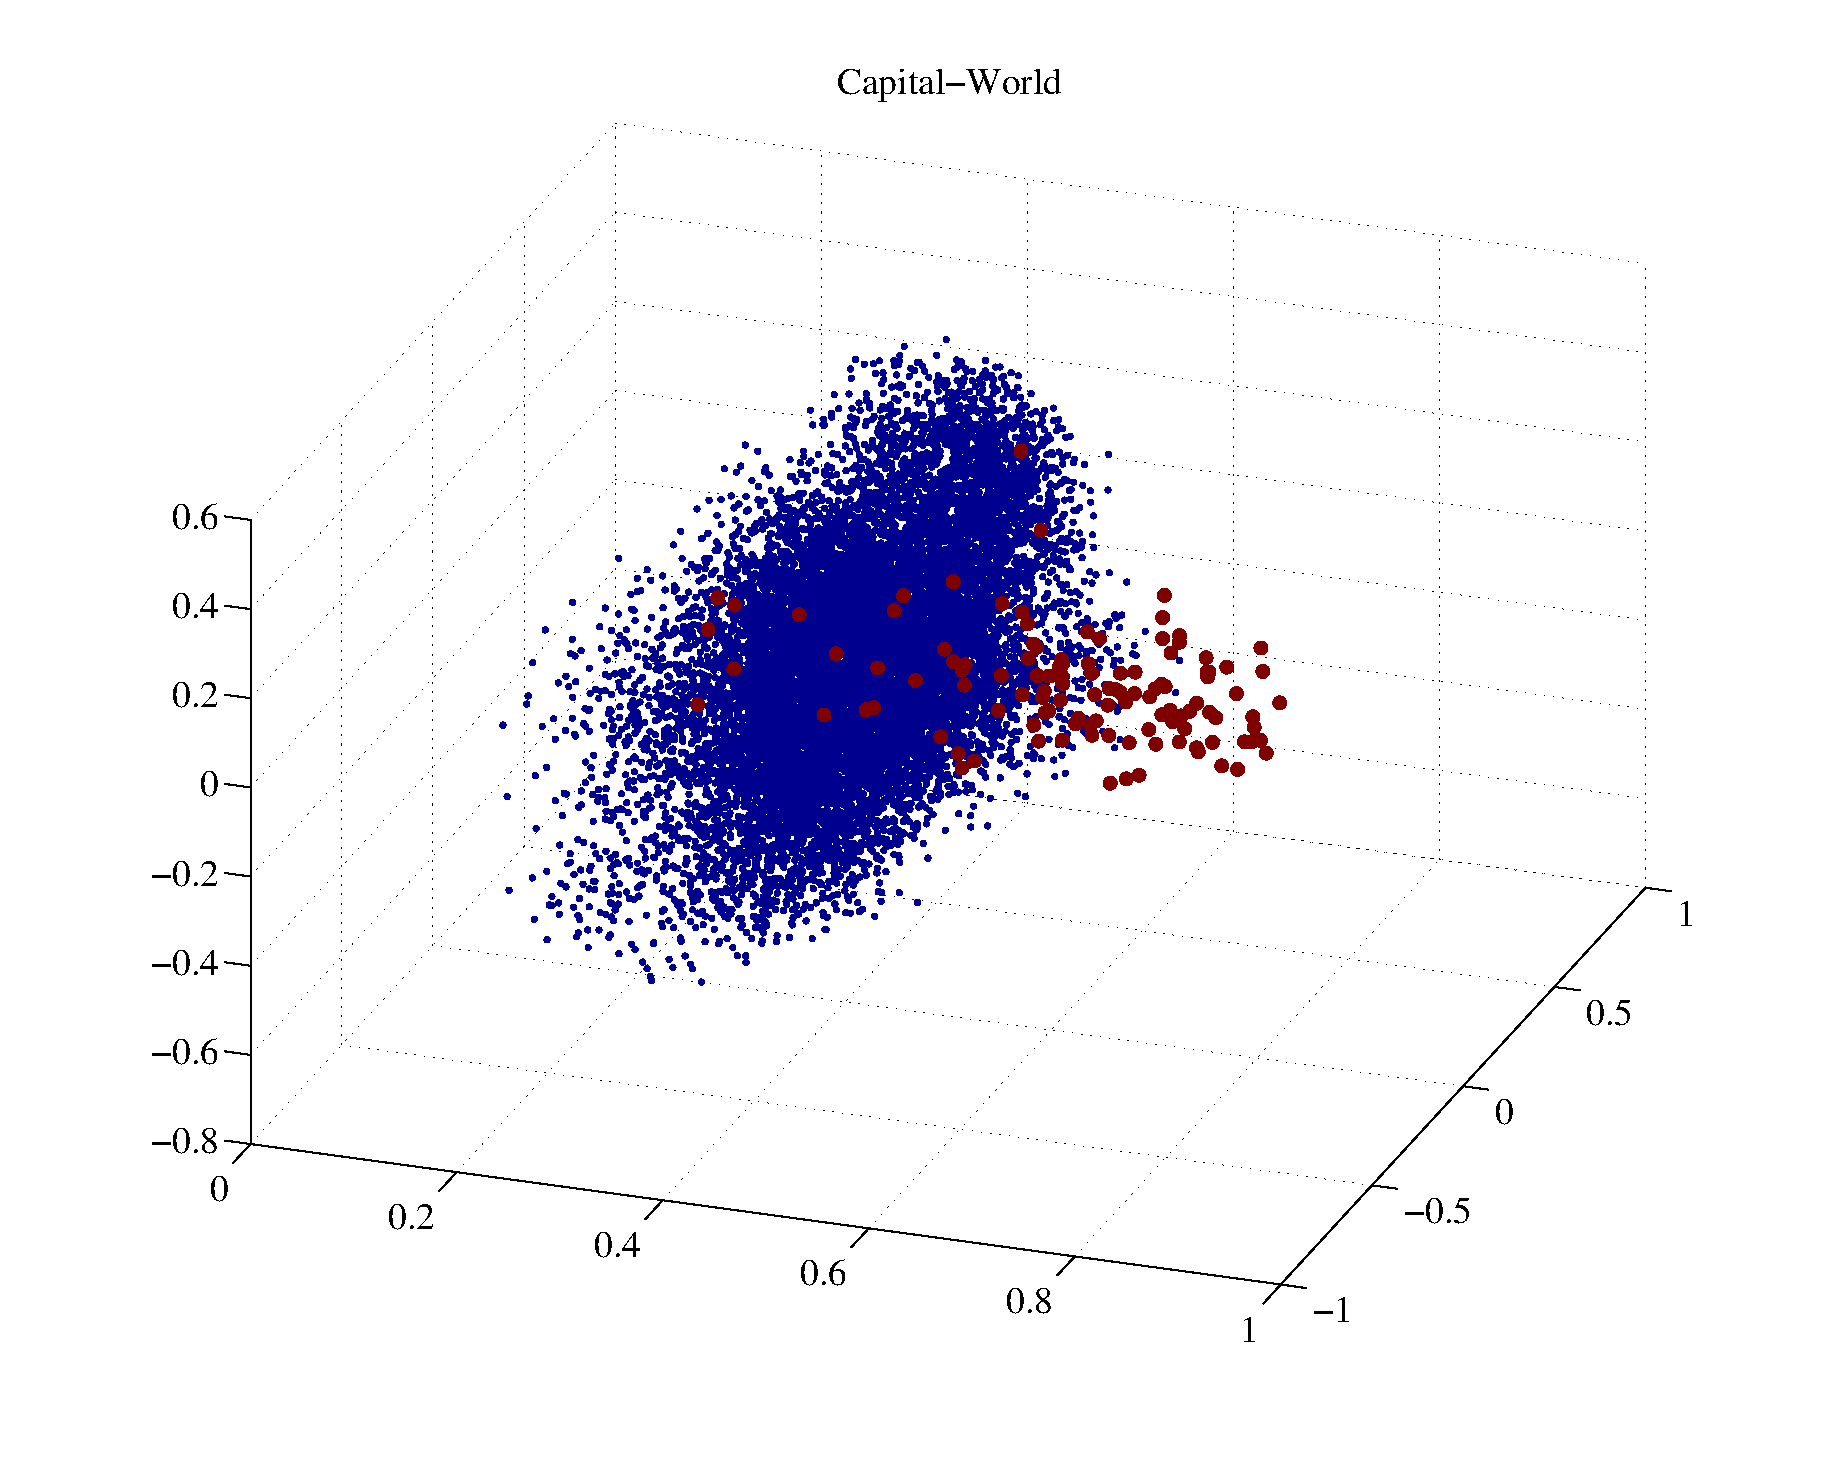
\includegraphics[width=.45\textwidth]{./images/capital_world.eps}
}
\subfigure[Nationality-Adjective]{
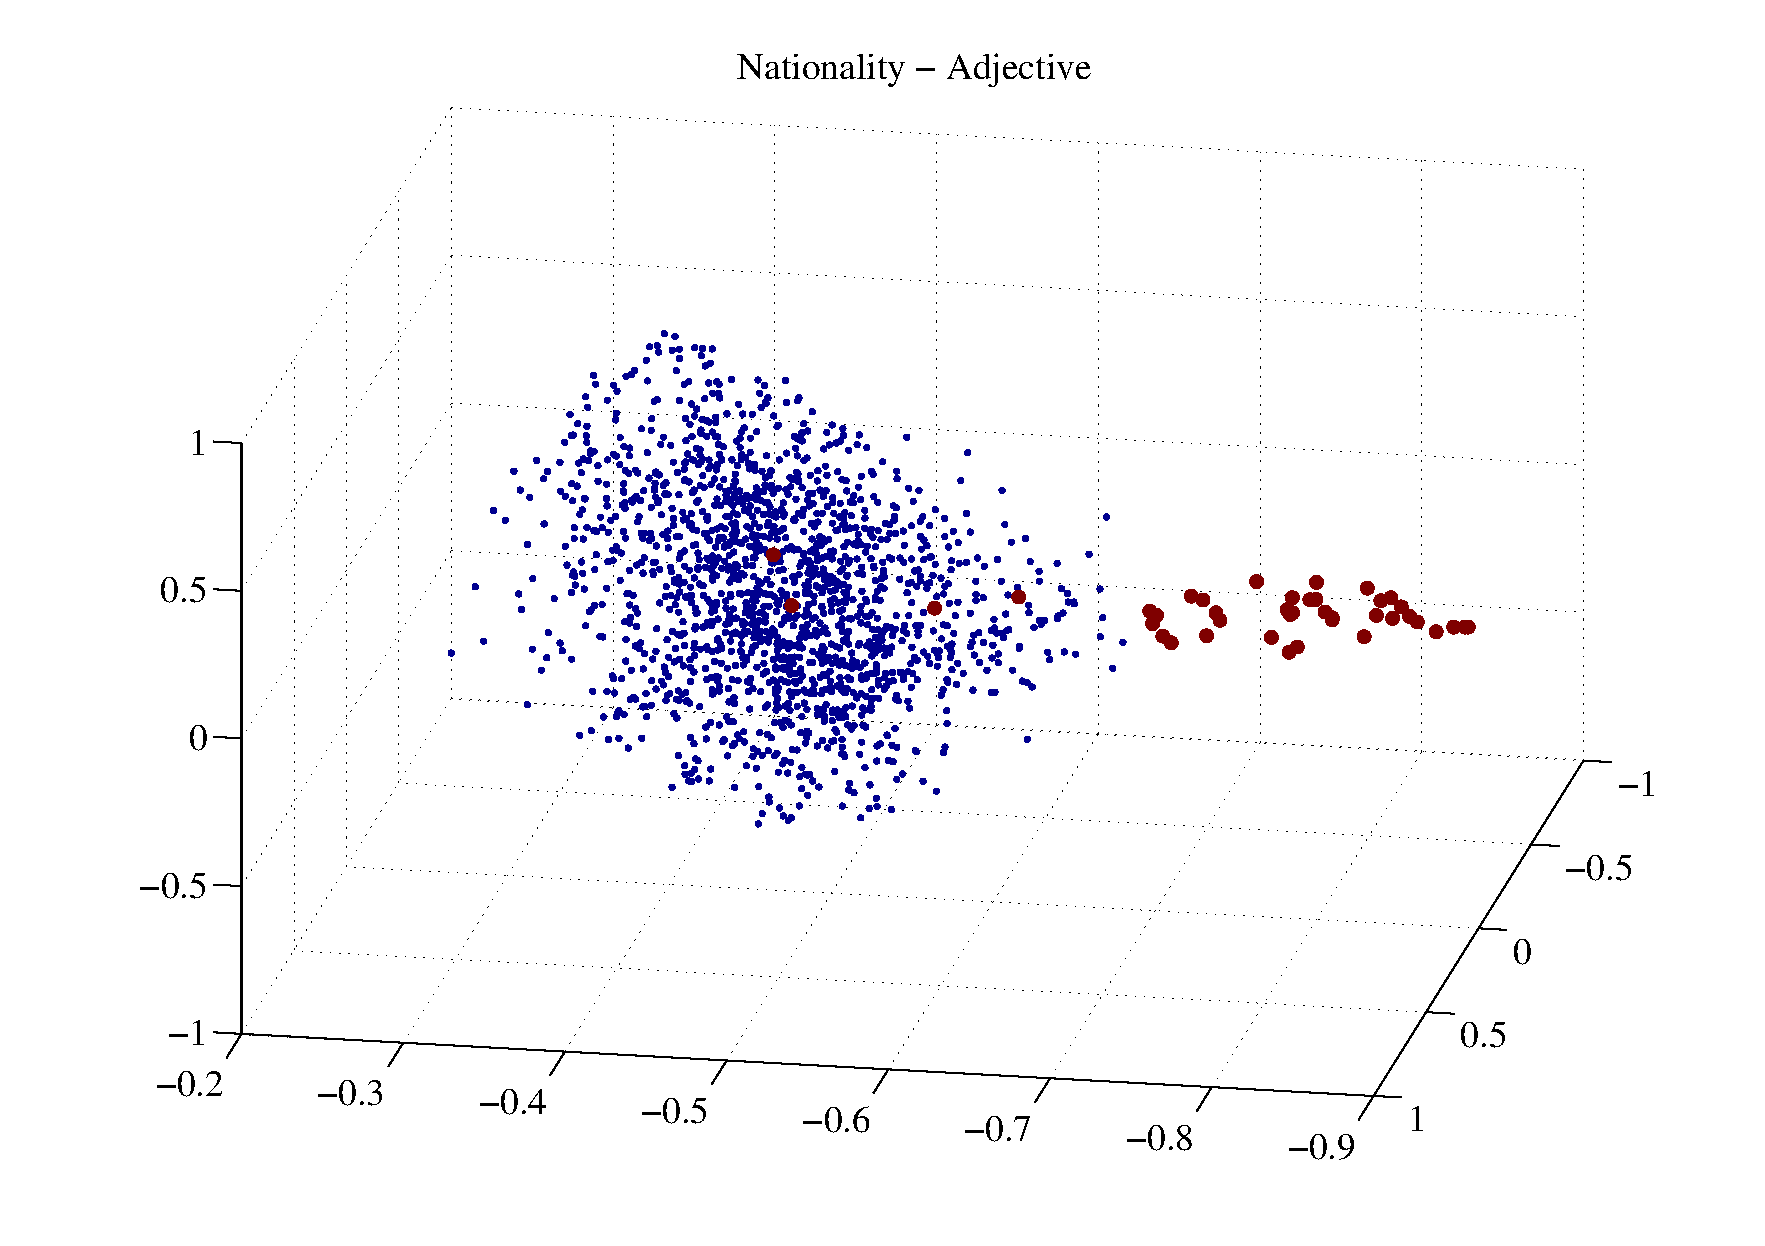
\includegraphics[width=.45\textwidth]{./images/nationality_adj.eps}
}

\subfigure[Plural-Vebs]{
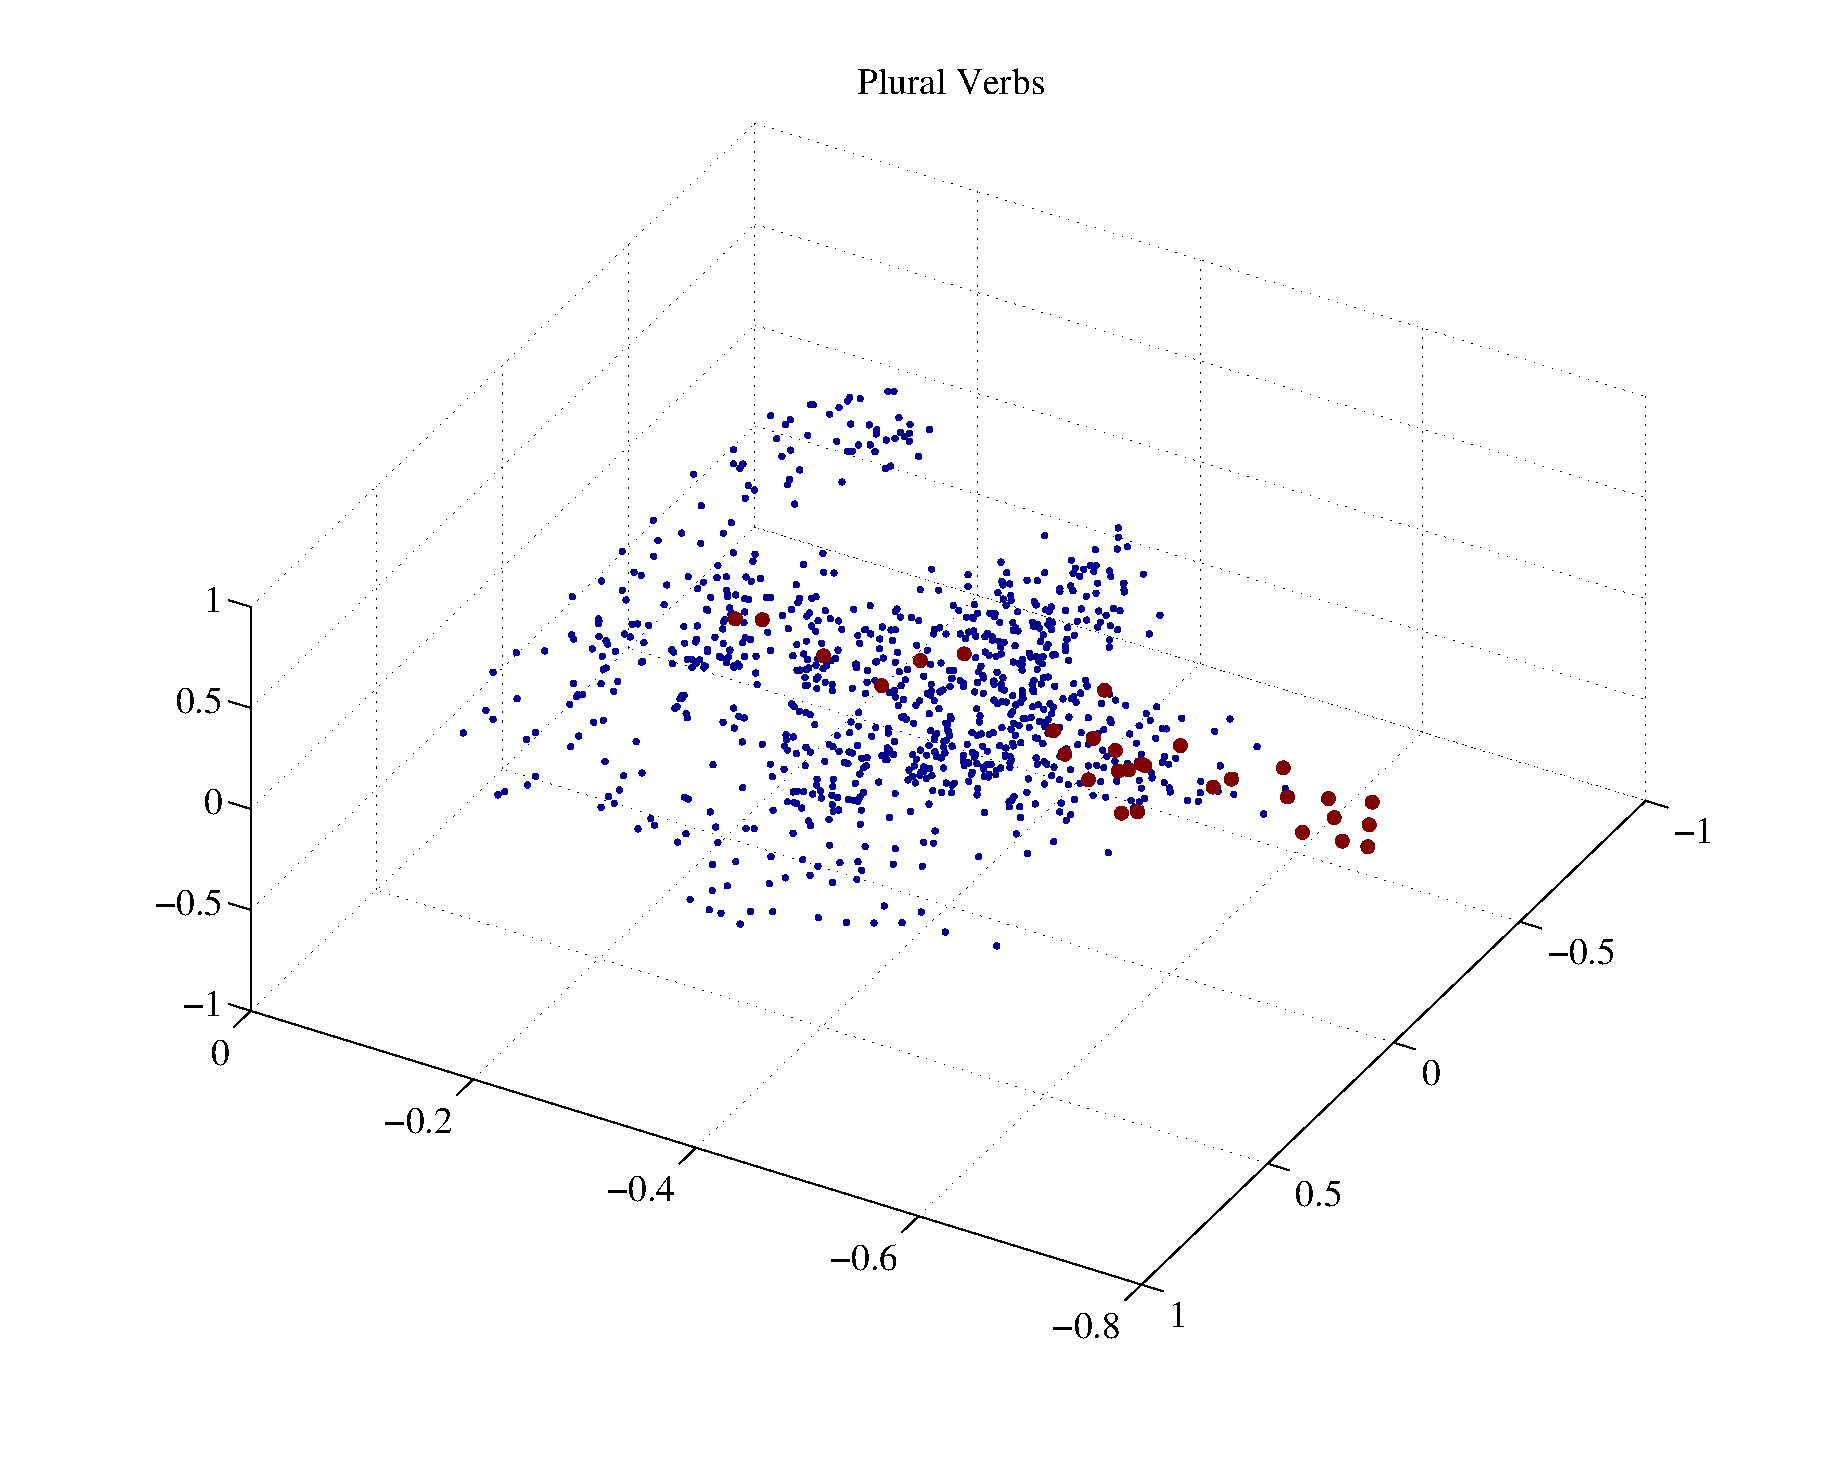
\includegraphics[width=.45\textwidth]{./images/plural_verbs.eps}
}
\caption{Projections of Vector Offsets for different categories of Word-Pairs}
\label{fig:offsetProj}
\end{figure}

\subsection{Low rank approximations of word vectors}
Ideally, we would like to be able to fit a variety of subspaces to all the word vectors. However, in practice the number of word vectors in our embedding space may be too large to afford running a subspace clustering algorithm on the entire set. To with this problem, we generate sets of words related by a high level concept and explore how well the word vectors associated with the set is approximated by a rank $k$ subspace, for varying $k$. If the set of vectors is well approximated by a rank $k$ subspace, for $k$ smaller than the original dimension of the space, then we can conclude the set of word vectors does in fact have linear low dimensional structure. Figure \ref{fig:svdOnClass} shows rank versus the $L2$ approximation error for word vectors in a variety of classes. As the figure shows, some classes are much more amenable to low rank approximations than others. This may partially be a product of our method generating related words (currently being done via a search of the WordNet hierarchy). 


\begin{figure}[t]
\centering
\includegraphics[width=.65\textwidth]{./images/svd_per_class.eps}
\caption{Rank vs. $L2$ error for different sets of word vectors}
\label{fig:svdOnClass}
\end{figure}

\subsection{Exploring planar structure of analogical pairs}
In an attempt to gain some insight into the embedding space we did the following: 
\begin{enumerate}
  \item Take 3 words from one of the cases in the analogical reasoning test set and compute the subspace that best fits the corresponding word vectors.
  \item Project all word vectors onto this plane.
  \item Throw away all vectors greater than some threshold away from the plane (in the examples plotted below we kept only the closest 20 vectors)
  \item Plot the remaining word vectors projected onto the plane, coded (by size where large indicates a greater distance) based on their distance from the plane. 
  \item Highlight points that would be predicted (using the projected vectors) within the top $k$ (we used $k = 5$) using the vector offset method.
\end{enumerate}

\begin{figure}[t]
\centering
\subfigure[Greece : Athens - Thailand : Bangkok]{
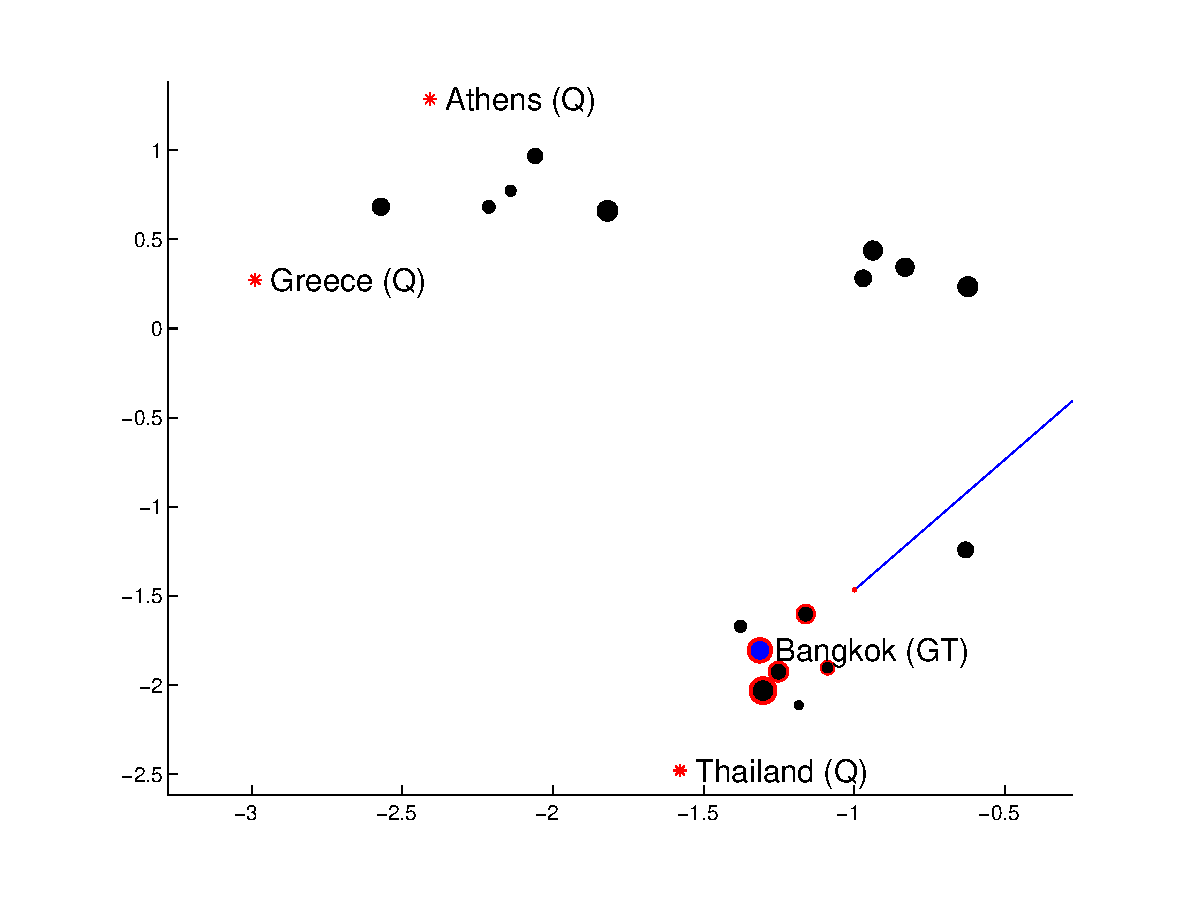
\includegraphics[width=.45\textwidth]{./images/greece_athens_thailand_bangkok.eps}
}
\subfigure[Greece : Athens - Japan : Tokyo]{
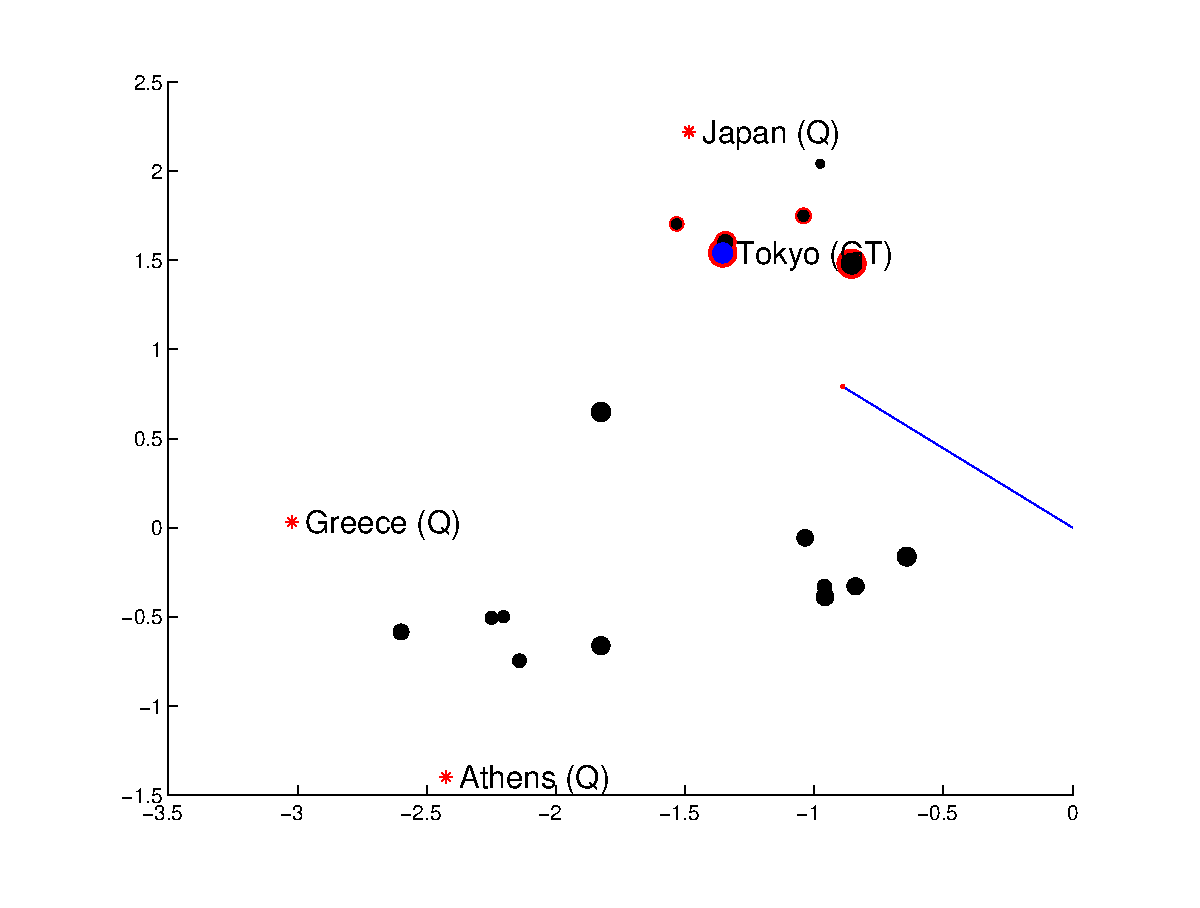
\includegraphics[width=.45\textwidth]{./images/greece_athens_japan_tokyo.eps}
}

\subfigure[Greece : Athens - Russia : Moscow]{
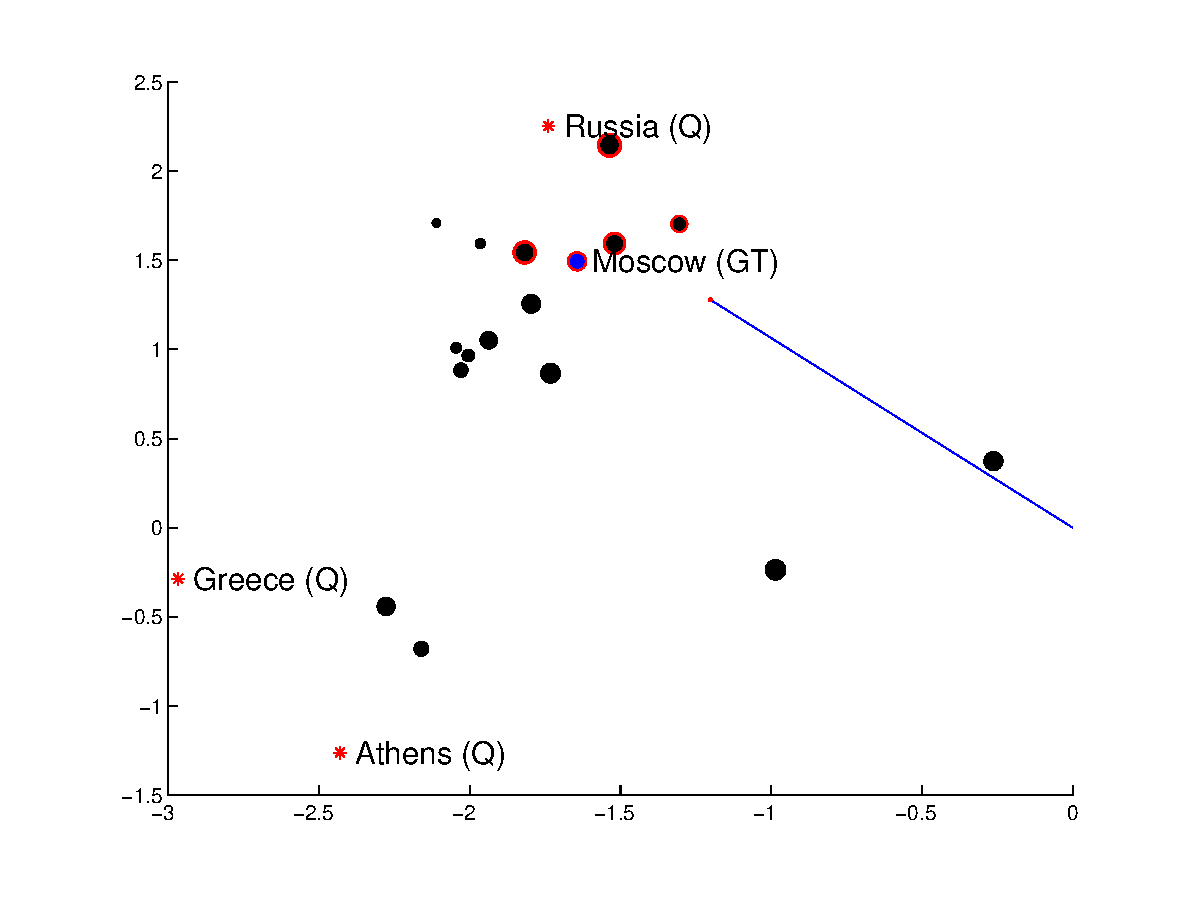
\includegraphics[width=.45\textwidth]{./images/greece_athens_russia_moscow.eps}
}
\subfigure[Greece : Athens - Egypt : Cairo]{
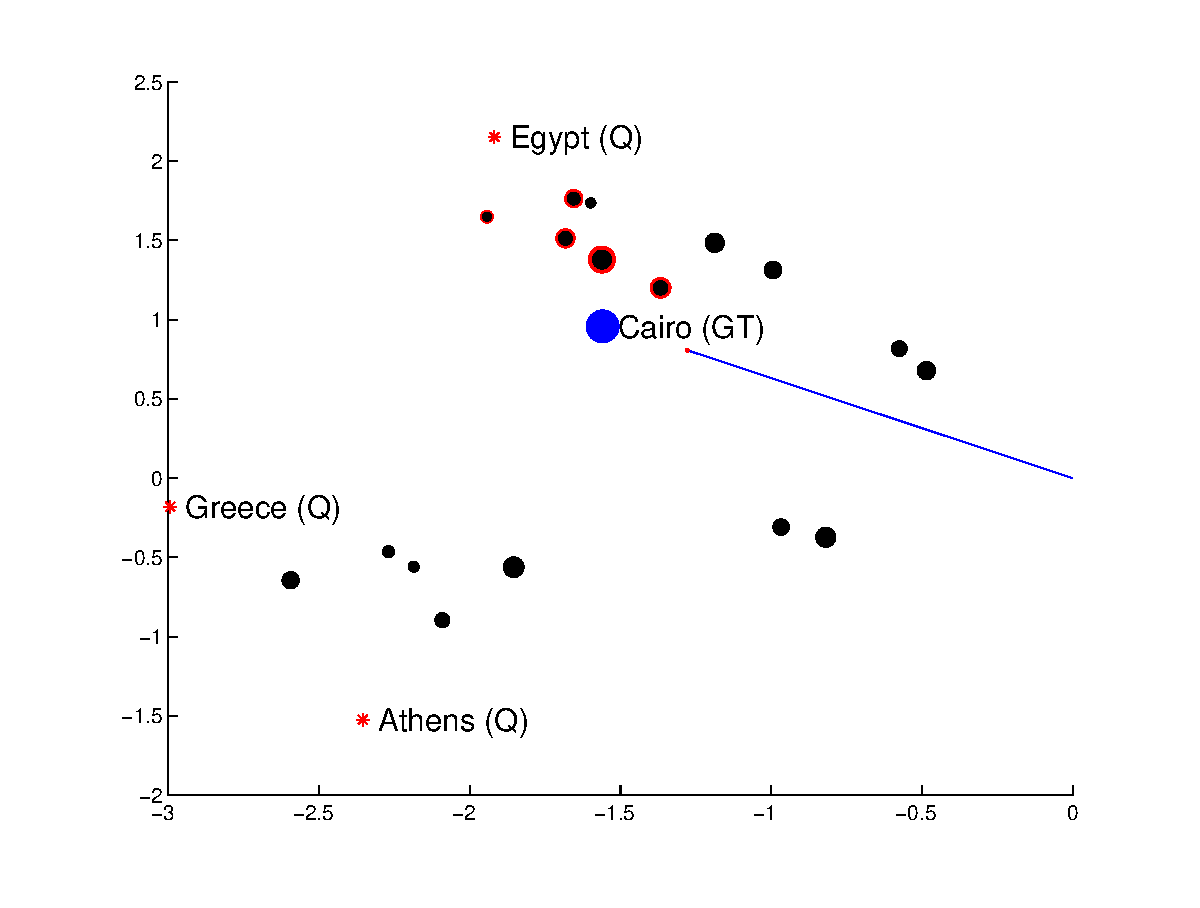
\includegraphics[width=.45\textwidth]{./images/greece_athens_egypt_cairo.eps}
}
\caption{Analogical reasoning word vectors projected onto 2D plane}
\label{fig:offsetProj}
\end{figure}

\clearpage


\subsection{Comparing Models} 
In this section, we compare the different models based on their top 5 accuracy on the different sections of the analogical reasoning test. 

Additionally, we depict the values of the 


\section{Conclusion}
\nocite{*}
\bibliographystyle{splncs}
\bibliography{bibliography}

\end{document}
